\documentclass[11pt]{article}

\usepackage{amsmath,amssymb}
\usepackage{booktabs}
\usepackage{caption}
\usepackage{fontspec}
\usepackage[margin=1in]{geometry}
\usepackage{graphicx}
\usepackage{hyperref}
\usepackage{microtype}
\usepackage{xcolor}

\hypersetup{
  colorlinks=true,
  linkcolor=blue!55!black,
  urlcolor=blue!55!black,
  pdftitle={Particle-in-a-box residuals and identifiability},
  pdfauthor={ksdft2effmass project}
}
\graphicspath{{./}}
\setlength{\parindent}{0pt}
\setlength{\parskip}{0.65em}

\newcommand{\statusbox}[1]{%
  \begin{center}
  \fcolorbox{black!55}{gray!8}{%
    \begin{minipage}{0.92\textwidth}
    \textbf{Evidence status.} #1
    \end{minipage}}
  \end{center}}

\title{Particle-in-a-Box Residuals and Identifiability\\
\large Provisional Experiment Report and Draft Appendix D}
\author{\texttt{ksdft2effmass} research workspace}
\date{}

\begin{document}
\maketitle

\statusbox{Calculated illustrative numerical experiment and provisional
manuscript draft. This document is not a reviewed manuscript, released research
result, semiconductor calculation, scientific validation result, or
uncertainty-quantification study.}

\begin{abstract}
The one-dimensional particle in a box provides a closed-form setting in which a
continuum operator, its domain, a finite representation, spectral retention,
and reduced-model interpretation can be kept distinct. This report tests three
matrix residuals that could otherwise be conflated under the label of an
effective potential. Consistent compression of the Dirichlet Hamiltonian and
kinetic operator gives zero potential. Compressing only the Hamiltonian produces
the negative discarded kinetic sector. Subtracting a cyclic finite-space
reference produces a boundary-realization difference.

Grid-refinement calculations over $N=8,16,32,64,128,256$ interior points verify
second-order convergence for fixed eigenvalue indices. A full-spectrum sweep
shows that this convergence is not uniform when mode index grows with grid
dimension. Frobenius, spectral, and maximum-entry norm studies show that a
residual can become small in an aggregate same-grid norm while remaining
significant in a worst-case norm. Finally, two distinct exact decompositions of
the same retained Hamiltonian and four model-class fits demonstrate the central
identifiability result: a reduced Hamiltonian does not select a unique
kinetic--potential decomposition. A reference operator and admissible model
class must be specified before a residual receives a physical interpretation.
\end{abstract}

\tableofcontents
\clearpage

\section{Purpose}

The purpose is not to solve a difficult spectrum. The spectrum is known in
closed form. The purpose is to separate five ingredients that are easily mixed
in a more complicated reduction:
\begin{enumerate}
  \item the continuum Hamiltonian and its domain;
  \item the finite numerical representation;
  \item the full and retained state spaces;
  \item the projection and embedding maps; and
  \item the physical interpretation assigned to a residual.
\end{enumerate}

The controlled example asks what can be concluded from a subtraction such as
\begin{equation}
  H_{\mathrm{eff}}-T.
\end{equation}
The answer depends on which Hamiltonian and kinetic reference are used, whether
they act on the same space, whether both passed through the same reduction map,
and which potential model class is admissible. Numerical convergence alone does
not answer those questions.

\section{Continuum operator and finite realization}

For a particle of mass $m$ on $(0,L)$, the continuum reference is the
Dirichlet realization
\begin{equation}
  \hat H_{\mathrm{box}}
  =-\frac{\hbar^2}{2m}\frac{d^2}{dx^2},
  \qquad
  \mathcal D(\hat H_{\mathrm{box}})=H^2(0,L)\cap H_0^1(0,L).
\end{equation}
The boundary conditions are $\psi(0)=\psi(L)=0$. The eigenpairs are
\begin{equation}
  \psi_n(x)=\sqrt{\frac{2}{L}}\sin\!\left(\frac{n\pi x}{L}\right),
  \qquad
  E_n=\frac{\hbar^2\pi^2n^2}{2mL^2}.
\end{equation}
The interior physical potential is zero. Confinement is represented by the
domain of the Dirichlet kinetic operator rather than by a finite-valued
multiplication potential inside the interval. This distinction is essential:
the differential expression alone does not define the self-adjoint operator,
and changing the boundary condition changes the operator even when the formal
kinetic expression is unchanged~\cite{bonneau2001,angelone2024}.

For $N$ interior points and spacing $h=L/(N+1)$, the finite coordinate space is
$\mathcal V_h\cong\mathbb R^N$. The centered second-order realization is
\begin{equation}
\mathbf H_h
=
\frac{\hbar^2}{2mh^2}
\begin{bmatrix}
2 & -1 & 0 & \cdots & 0\\
-1 & 2 & -1 & \ddots & \vdots\\
0 & -1 & 2 & \ddots & 0\\
\vdots & \ddots & \ddots & \ddots & -1\\
0 & \cdots & 0 & -1 & 2
\end{bmatrix}.
\end{equation}
The calculated experiments use the dimensionless convention $L=m=\hbar=1$.
The centered stencil is a second-order finite-difference approximation in the
usual local truncation sense~\cite{strikwerda2004}. For this particular Toeplitz
matrix, the complete discrete spectrum is also available analytically:
\begin{equation}
  E_{n,h}
  =\frac{2\hbar^2}{mh^2}
   \sin^2\!\left(\frac{n\pi}{2(N+1)}\right),
  \qquad n=1,\ldots,N.
\end{equation}
This formula supplies an oracle independent of the numerical eigensolver and
makes it possible to distinguish discretization error from algebraic solution
error throughout the report.

\section{Spectral retention and state-space maps}

Let $\boldsymbol\Phi_M\in\mathbb R^{N\times M}$ contain the lowest $M$
orthonormal eigenvectors of $\mathbf H_h$. Define
\begin{equation}
  \mathbf P_M=\boldsymbol\Phi_M\boldsymbol\Phi_M^T,
  \qquad
  \mathbf Q_M=\mathbf I-\mathbf P_M.
\end{equation}
Two representations of the retained operator are needed:
\begin{align}
  \mathbf H_h^{(P_M)}
  &=\mathbf P_M\mathbf H_h\mathbf P_M
  \in\mathbb R^{N\times N},\\
  \mathbf H_{\mathrm{red}}
  &=\boldsymbol\Phi_M^T\mathbf H_h\boldsymbol\Phi_M
  \in\mathbb R^{M\times M}.
\end{align}
The first is an embedded rank-$M$ matrix on the full numerical space. The second
is the same retained operator in retained spectral coordinates. Their
dimensions differ, so an embedding must be declared before comparison.

For the retained $N=8$, $M=3$ calculation, the numerical checks were:
\begin{table}[htbp]
\centering
\caption{Finite-representation diagnostics.}
\begin{tabular}{lr}
\toprule
Diagnostic & Calculated value\\
\midrule
Discrete spectrum maximum absolute oracle error & $8.53\times10^{-14}$\\
Spectral reconstruction Frobenius error & $3.04\times10^{-13}$\\
Projector idempotency Frobenius error & $8.48\times10^{-16}$\\
Retained-coordinate Frobenius error & $2.46\times10^{-14}$\\
Retained embedding Frobenius error & $1.02\times10^{-14}$\\
\bottomrule
\end{tabular}
\end{table}

\begin{figure}[p]
\centering
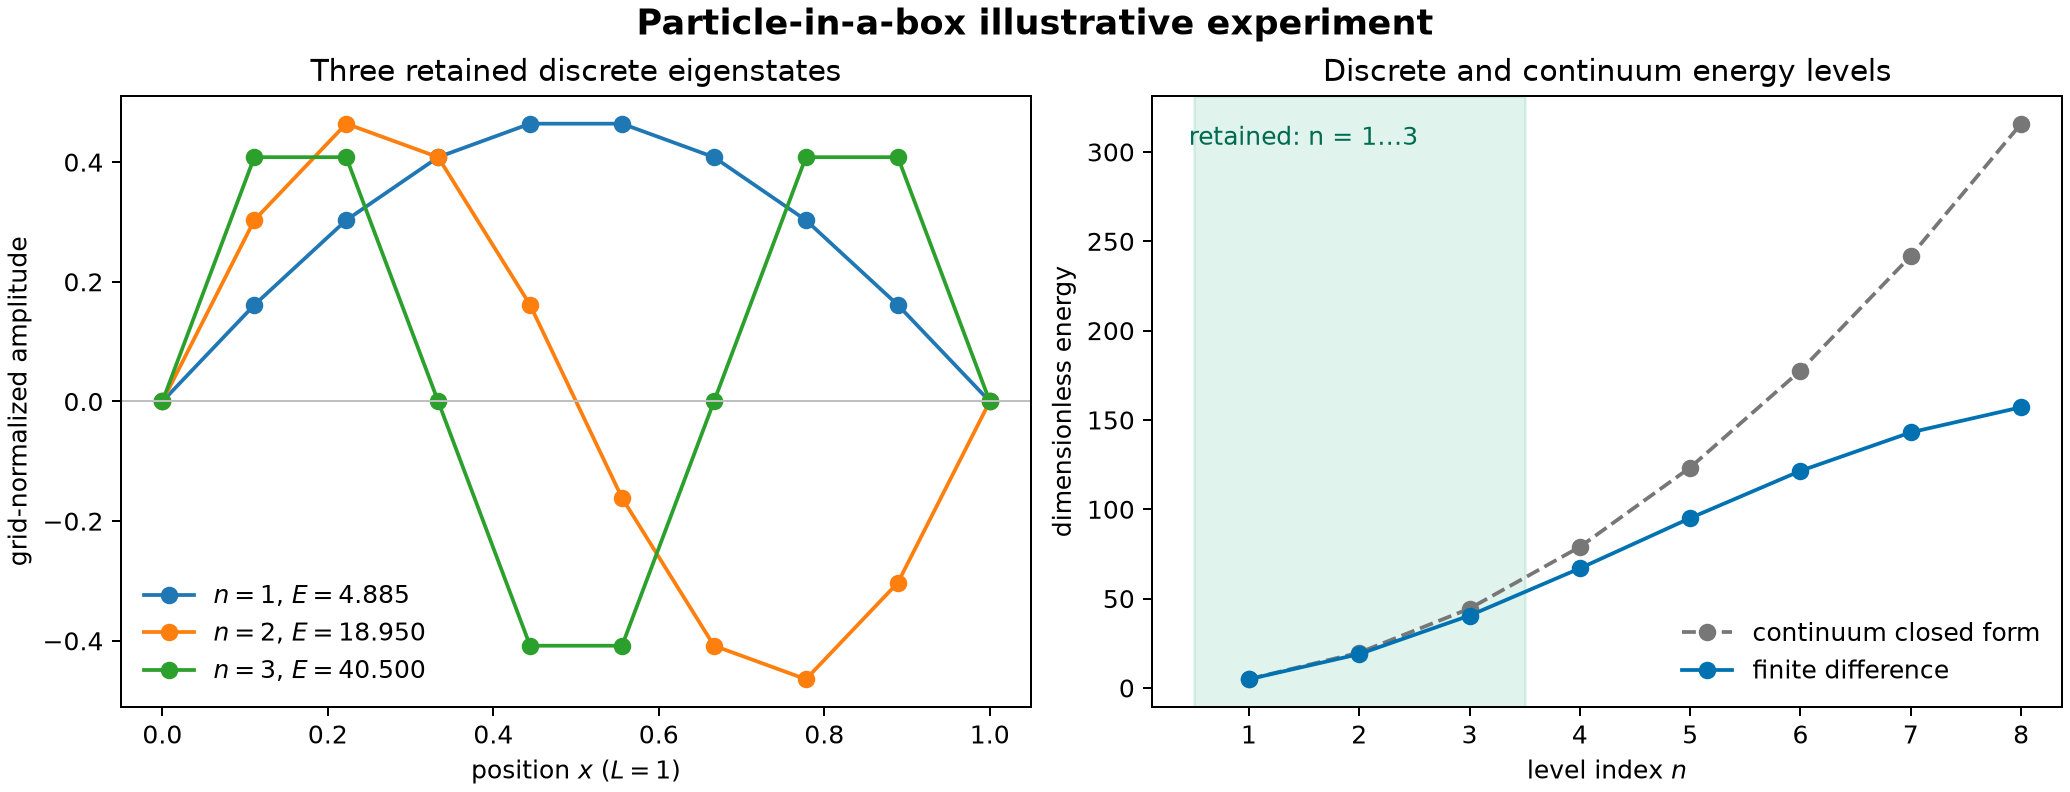
\includegraphics[width=\textwidth]{spectrum-and-states.png}
\caption{The three retained states and the finite and continuum spectra. The
finite grid underestimates increasingly high continuum energies.}
\label{fig:states-spectrum}
\end{figure}

\section{Three inequivalent residuals}

\subsection{Consistently compressed physical potential}

In this model, $\mathbf H_h=\mathbf T_{\mathrm D,h}$. Applying the same
compression to both terms gives
\begin{equation}
  \mathbf P_M\mathbf H_h\mathbf P_M
  -\mathbf P_M\mathbf T_{\mathrm D,h}\mathbf P_M
  =\mathbf0.
\end{equation}
The calculated Frobenius norm is exactly zero. This is the consistently reduced
physical potential for the declared box model.

\subsection{Compressed Hamiltonian minus uncompressed kinetic operator}

If only the Hamiltonian is compressed,
\begin{equation}
  \widetilde{\mathbf R}_h
  =\mathbf P_M\mathbf H_h\mathbf P_M-\mathbf T_{\mathrm D,h},
\end{equation}
then spectral commutation gives
\begin{equation}
  \widetilde{\mathbf R}_h
  =-\mathbf Q_M\mathbf T_{\mathrm D,h}\mathbf Q_M.
\end{equation}
For $N=8$ and $M=3$, the calculated Frobenius norm is $270.977$, and the
Frobenius error against the negative discarded-sector oracle is
$8.75\times10^{-14}$. The nonzero matrix is caused by unmatched reduction. It is
not the physical box potential.

\subsection{Difference between boundary realizations}

A cyclic closure was declared as a comparison reference on the same finite
coordinate space. The difference
\begin{equation}
  \mathbf B_h
  =\mathbf H_{\mathrm D,h}-\mathbf H_{\mathrm{cyclic},h}
\end{equation}
contains two corner couplings. At $N=8$, its Frobenius norm is $57.276$. This is
a finite boundary-realization difference relative to the declared cyclic
reference, not a representation-independent continuum potential.

\begin{figure}[p]
\centering
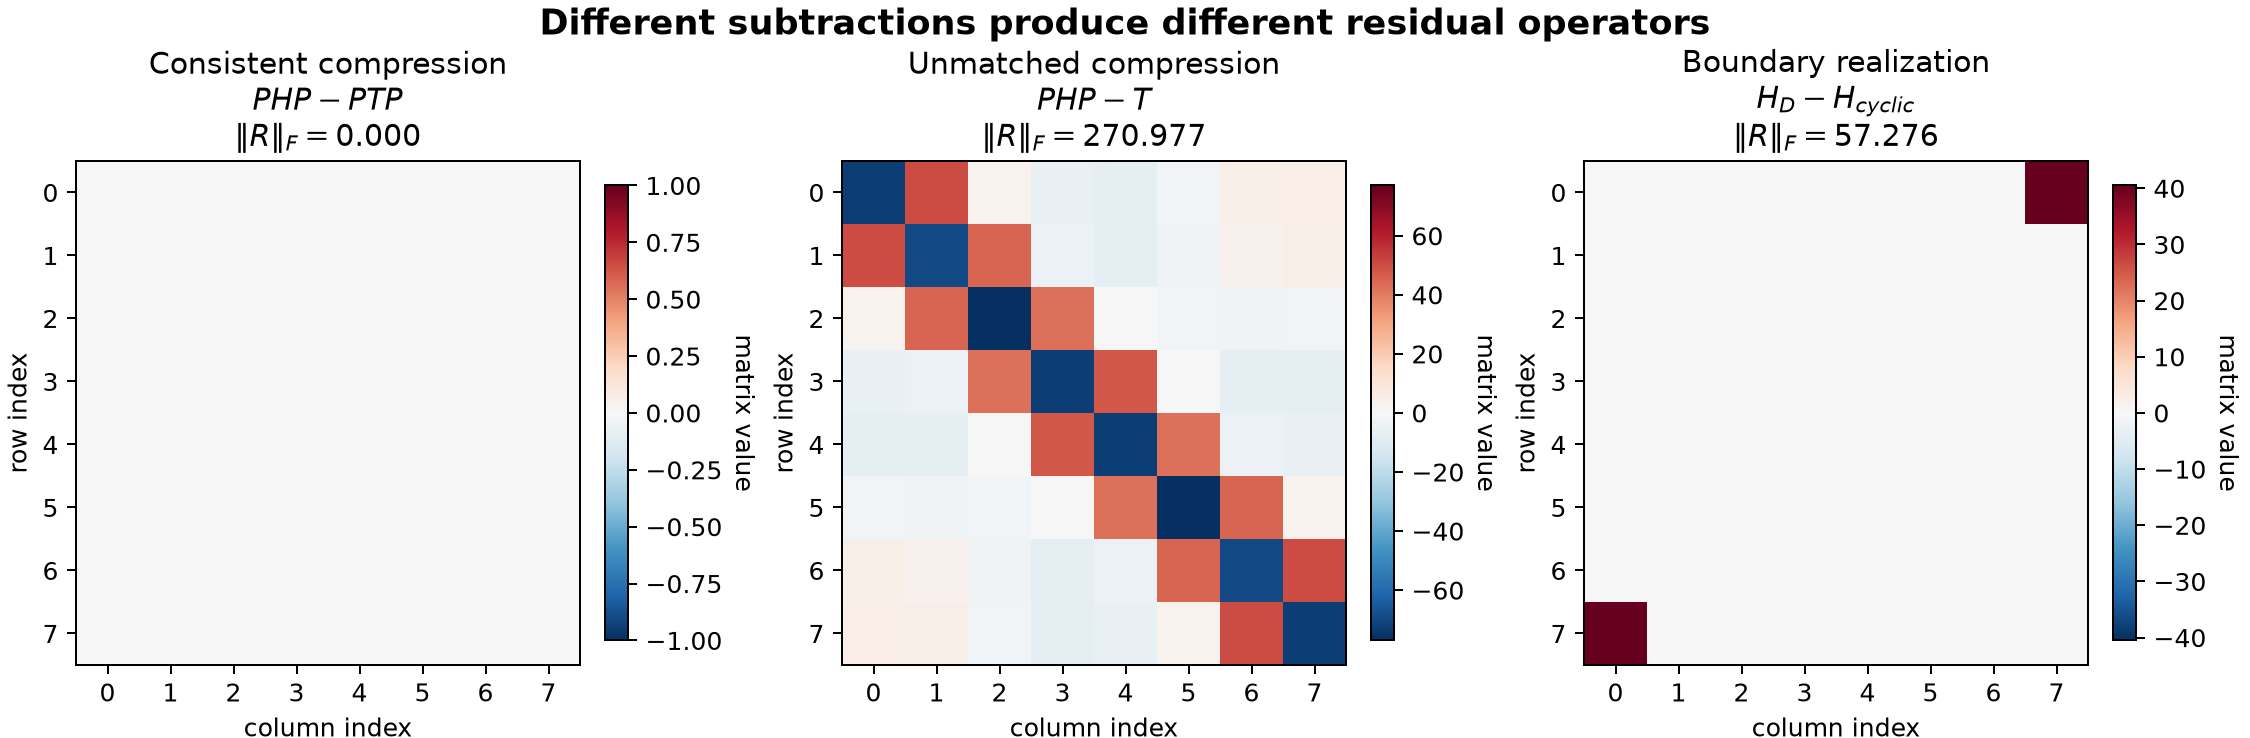
\includegraphics[width=\textwidth]{residual-matrices.png}
\caption{The three residual constructions. Identical subtraction syntax does
not imply identical mathematical or physical meaning.}
\label{fig:residuals}
\end{figure}

\clearpage
\section{Fixed-mode convergence}

The convergence study is retained because the finite representation must be
verified independently of residual interpretation. The grid sequence is
$N=8,16,32,64,128,256$. For each fixed mode, the relative energy error is
\begin{equation}
  \varepsilon_n(N)=\frac{|E_{n,h}-E_n|}{E_n}.
\end{equation}
Writing
\begin{equation}
  z_{n,N}=\frac{n\pi}{2(N+1)}=\frac{n\pi h}{2L},
\end{equation}
the exact ratio between the discrete and continuum eigenvalues is
\begin{equation}
  \frac{E_{n,h}}{E_n}
  =\left(\frac{\sin z_{n,N}}{z_{n,N}}\right)^2.
\end{equation}
For fixed $n$ and $h\to0$, Taylor expansion gives
\begin{equation}
  \varepsilon_n(N)
  =\frac{z_{n,N}^2}{3}+\mathcal O(z_{n,N}^4)
  =\frac{n^2\pi^2}{12L^2}h^2+\mathcal O(h^4).
\end{equation}
Thus the observed order-two trend is not merely empirical; it is the leading
term predicted by the exact dispersion relation. The coefficient grows as
$n^2$, explaining why higher fixed modes require finer grids before entering
the same asymptotic regime.

\subsection{Low fixed modes}

\begin{table}[htbp]
\centering
\caption{Relative energy errors for the first three fixed modes.}
\begin{tabular}{rrrr}
\toprule
$N$ & $n=1$ & $n=2$ & $n=3$\\
\midrule
8   & $1.0113\times10^{-2}$ & $3.9962\times10^{-2}$ & $8.8109\times10^{-2}$\\
16  & $2.8427\times10^{-3}$ & $1.1332\times10^{-2}$ & $2.5352\times10^{-2}$\\
32  & $7.5502\times10^{-4}$ & $3.0174\times10^{-3}$ & $6.7788\times10^{-3}$\\
64  & $1.9465\times10^{-4}$ & $7.7842\times10^{-4}$ & $1.7508\times10^{-3}$\\
128 & $4.9423\times10^{-5}$ & $1.9768\times10^{-4}$ & $4.4474\times10^{-4}$\\
256 & $1.2452\times10^{-5}$ & $4.9809\times10^{-5}$ & $1.1207\times10^{-4}$\\
\bottomrule
\end{tabular}
\end{table}

The final observed orders are 1.99998, 1.99991, and 1.99981 for $n=1,2,3$,
respectively. This is the expected second-order behavior for fixed resolved
modes.

\begin{figure}[p]
\centering
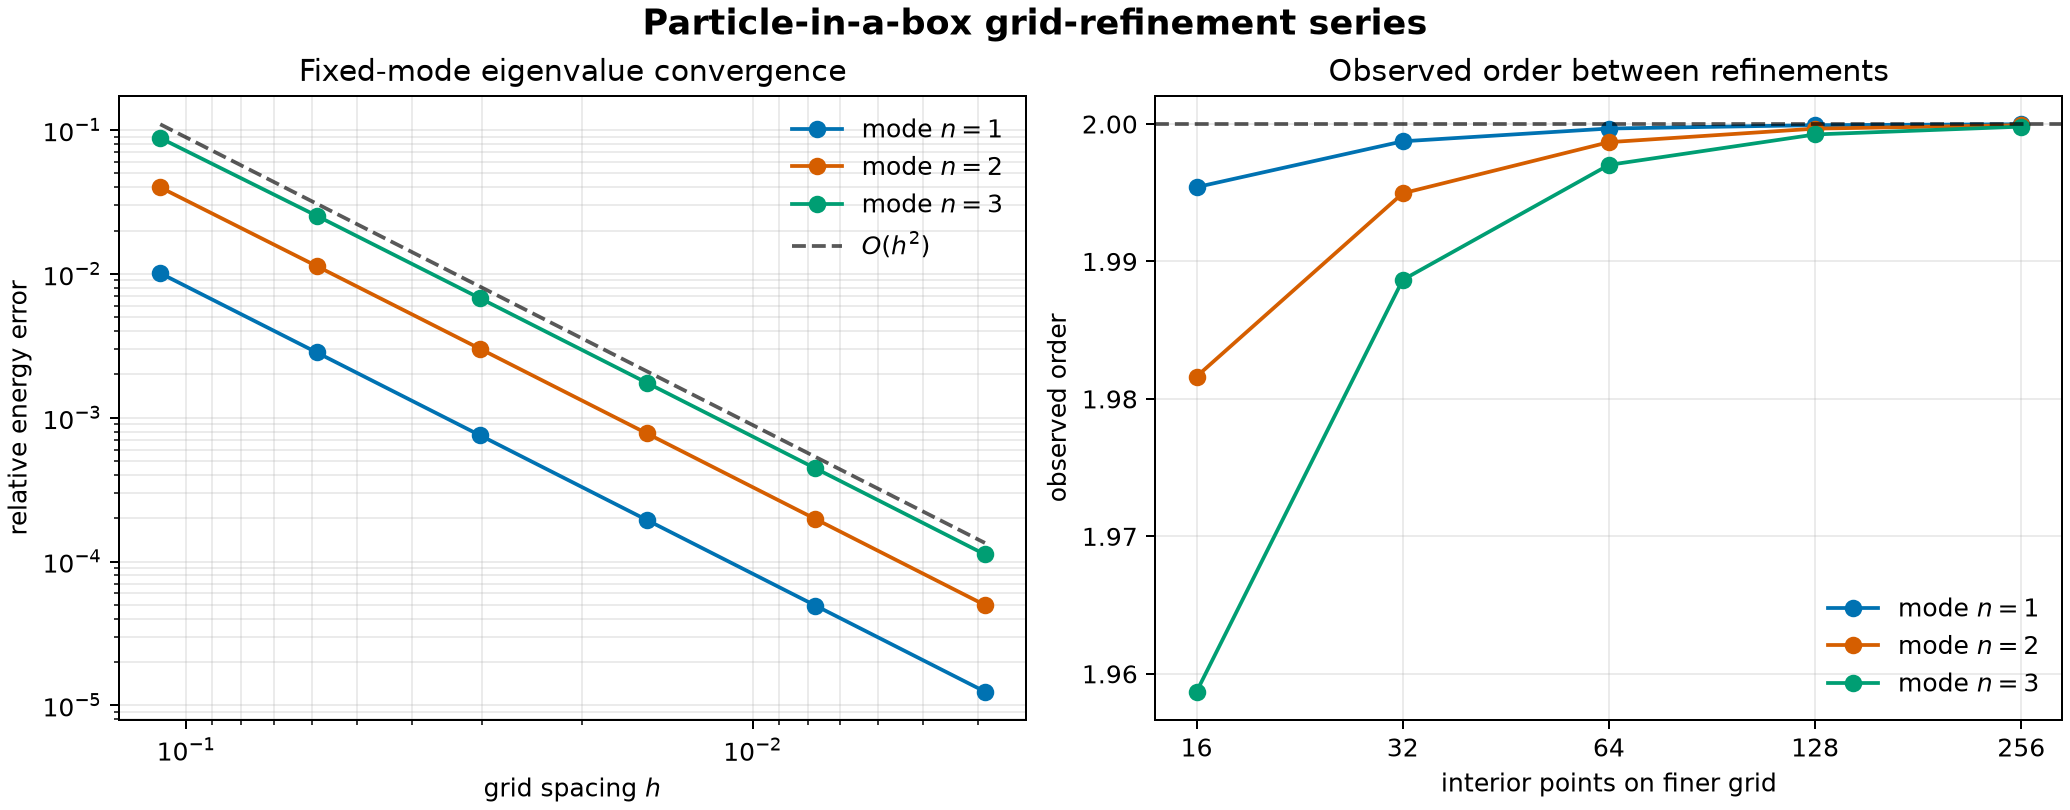
\includegraphics[width=\textwidth]{convergence-series.png}
\caption{Fixed low-mode relative errors and observed refinement orders.}
\label{fig:low-convergence}
\end{figure}

\begin{figure}[p]
\centering
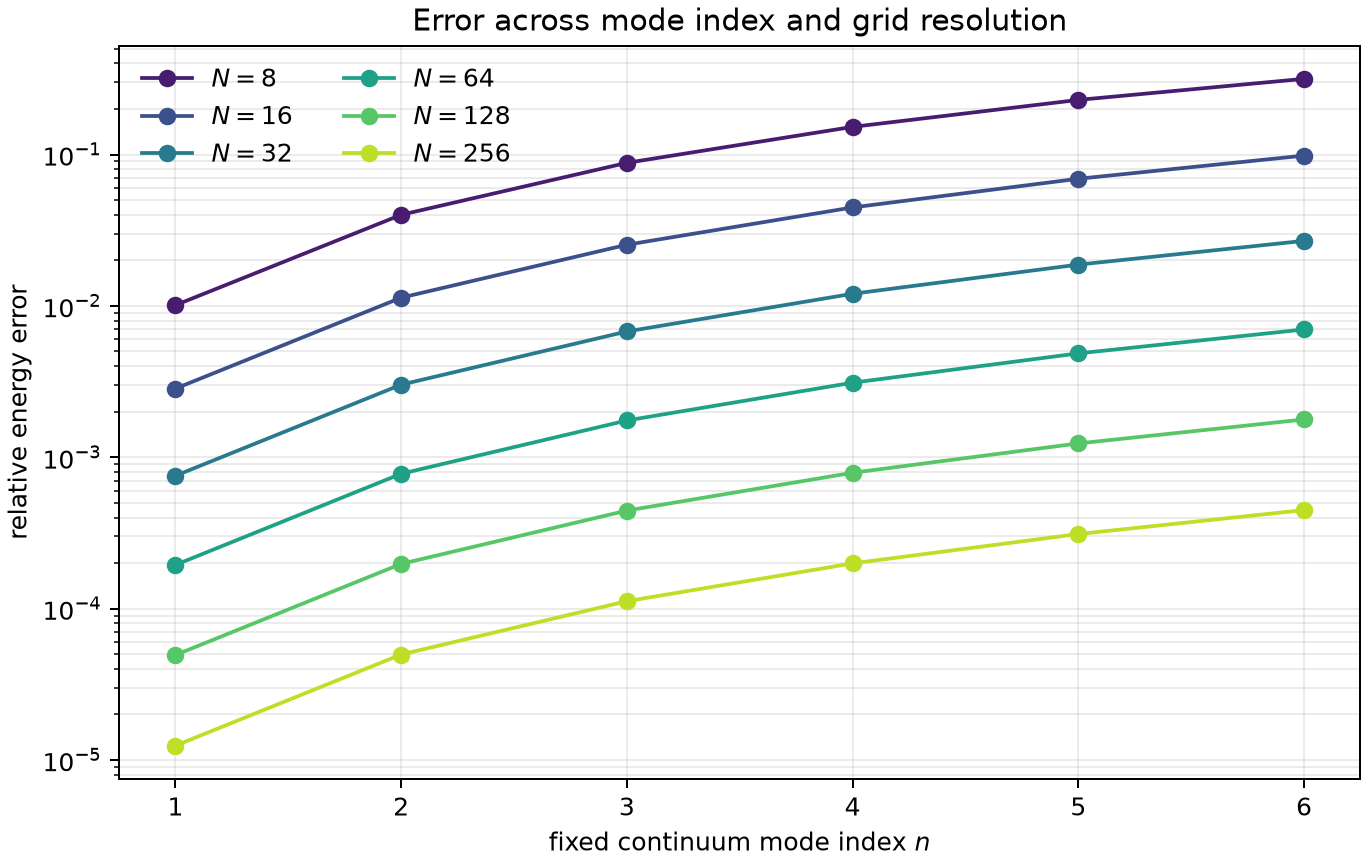
\includegraphics[width=0.88\textwidth]{convergence-mode-sweep.png}
\caption{Relative energy error across the first six fixed mode indices and the
full grid-refinement series.}
\label{fig:mode-sweep}
\end{figure}

\subsection{Fixed higher modes}

A fixed higher mode enters when it exists on the grid. The series starts at
$N=8$ for $n=8$, at $N=16$ for $n=16$, and at $N=32$ for $n=32$.

\begin{table}[htbp]
\centering
\caption{Convergence of fixed higher eigenvalues.}
\begin{tabular}{rrrr}
\toprule
Mode & First-grid relative error & $N=256$ relative error & Final order\\
\midrule
8  & $5.0253\times10^{-1}$ & $7.9670\times10^{-4}$ & 1.99863\\
16 & $5.4637\times10^{-1}$ & $3.1837\times10^{-3}$ & 1.99451\\
32 & $5.6997\times10^{-1}$ & $1.2686\times10^{-2}$ & 1.97805\\
\bottomrule
\end{tabular}
\end{table}

The initial points are under-resolved and pre-asymptotic. Each fixed mode moves
toward second-order behavior as the number of grid points per wavelength
increases.

\begin{figure}[p]
\centering
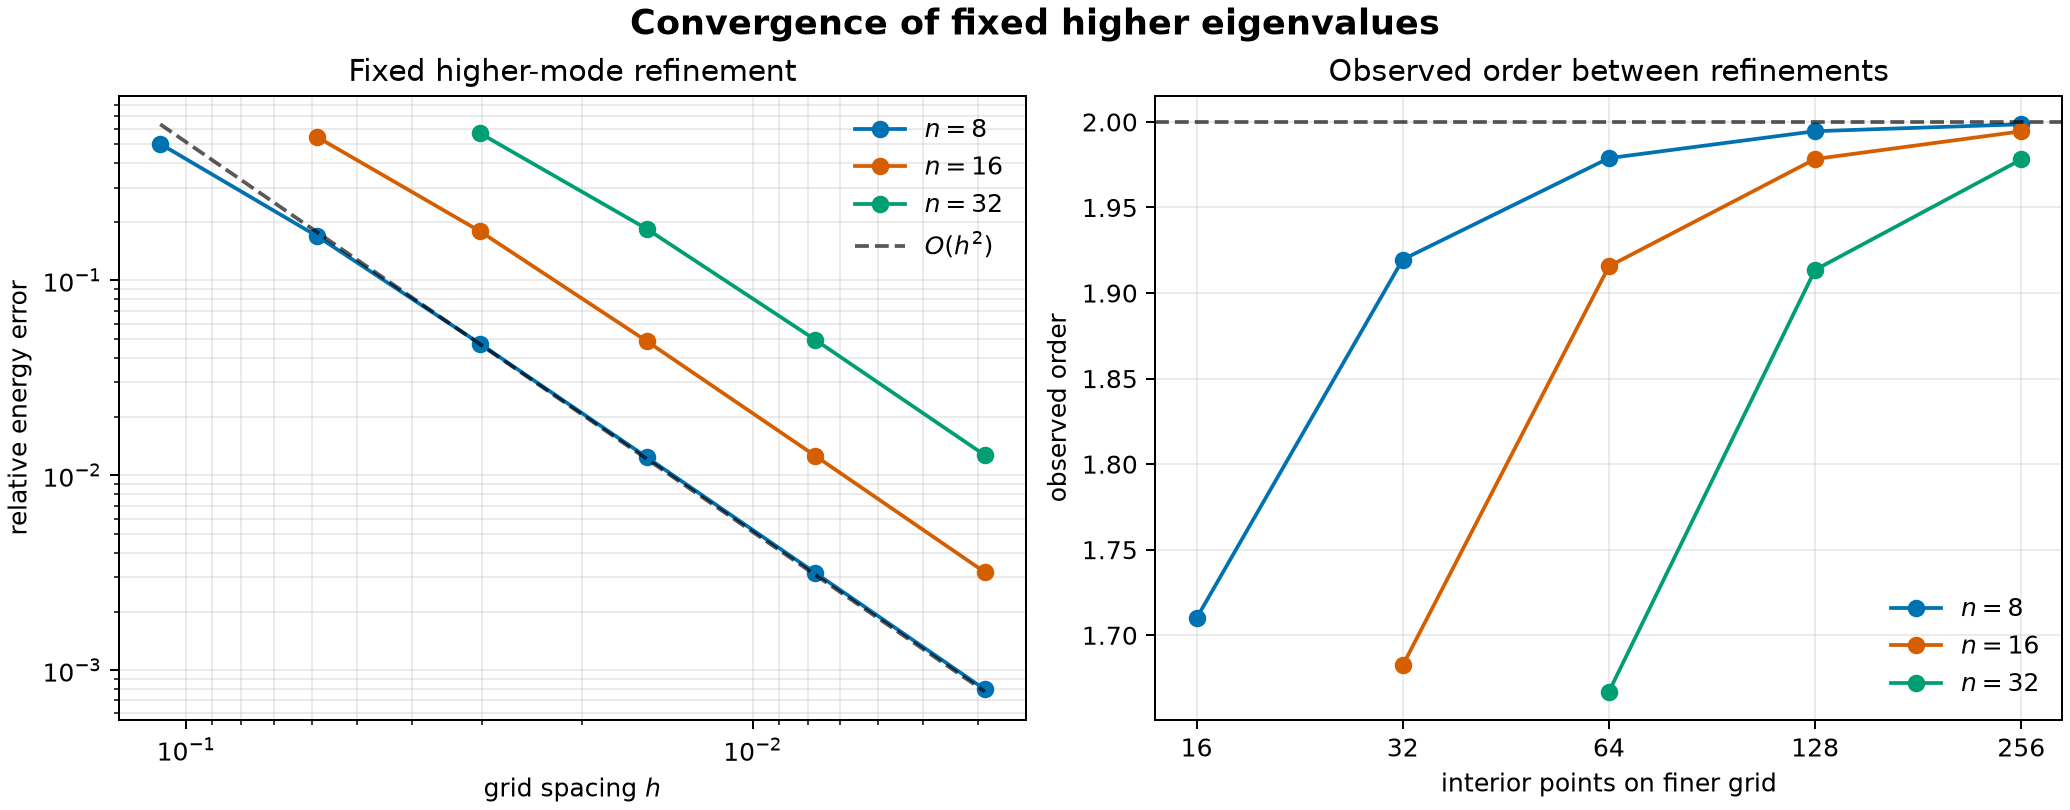
\includegraphics[width=\textwidth]{higher-mode-convergence.png}
\caption{Fixed higher-mode convergence and approach to second order.}
\label{fig:higher-convergence}
\end{figure}

\clearpage
\section{Full-spectrum eigenpair sweep}

Fixed-index convergence is not uniform spectral convergence. To expose that
distinction, the full discrete spectra were calculated for every grid from
$N=8$ through $N=256$. When the fractional mode index
\begin{equation}
  q=\frac{n}{N+1}
\end{equation}
is held approximately fixed, relative eigenvalue error remains substantial as
$N$ grows. Indeed, the exact eigenvalue ratio becomes
\begin{equation}
  \frac{E_{n,h}}{E_n}
  =
  \left[
    \frac{\sin(\pi q/2)}{\pi q/2}
  \right]^2.
\end{equation}
At fixed nonzero $q$, this expression is independent of $h$. Consequently the
relative error has a nonzero refinement limit. The full-spectrum curve collapse
is therefore an analytical feature of the stencil rather than a failure of the
eigensolver. Fixed-index convergence and convergence at fixed fractional mode
index are different limiting statements and must not be interchanged.

\begin{table}[htbp]
\centering
\caption{Representative full-spectrum errors at $N=256$.}
\begin{tabular}{rrr}
\toprule
$q$ & Mode & Relative energy error\\
\midrule
0.249 & 64  & $4.998\times10^{-2}$\\
0.498 & 128 & $1.881\times10^{-1}$\\
0.751 & 193 & $3.858\times10^{-1}$\\
0.996 & 256 & $5.916\times10^{-1}$\\
\bottomrule
\end{tabular}
\end{table}

The near-collapse of the curves as functions of $q$ is a finite-difference
dispersion result. Refining the grid improves each fixed physical mode, but it
does not make the entire growing discrete spectrum uniformly accurate.

At $N=256$, the maximum nodal overlap defect against sampled continuum sine
vectors is $4.00\times10^{-15}$, and the maximum scaled algebraic eigenpair
residual is $7.14\times10^{-16}$. These values show that the discrete
eigenpairs were solved accurately and agree with sine vectors at the nodes.
They do not measure error of an interpolated continuum wavefunction.

\begin{figure}[p]
\centering
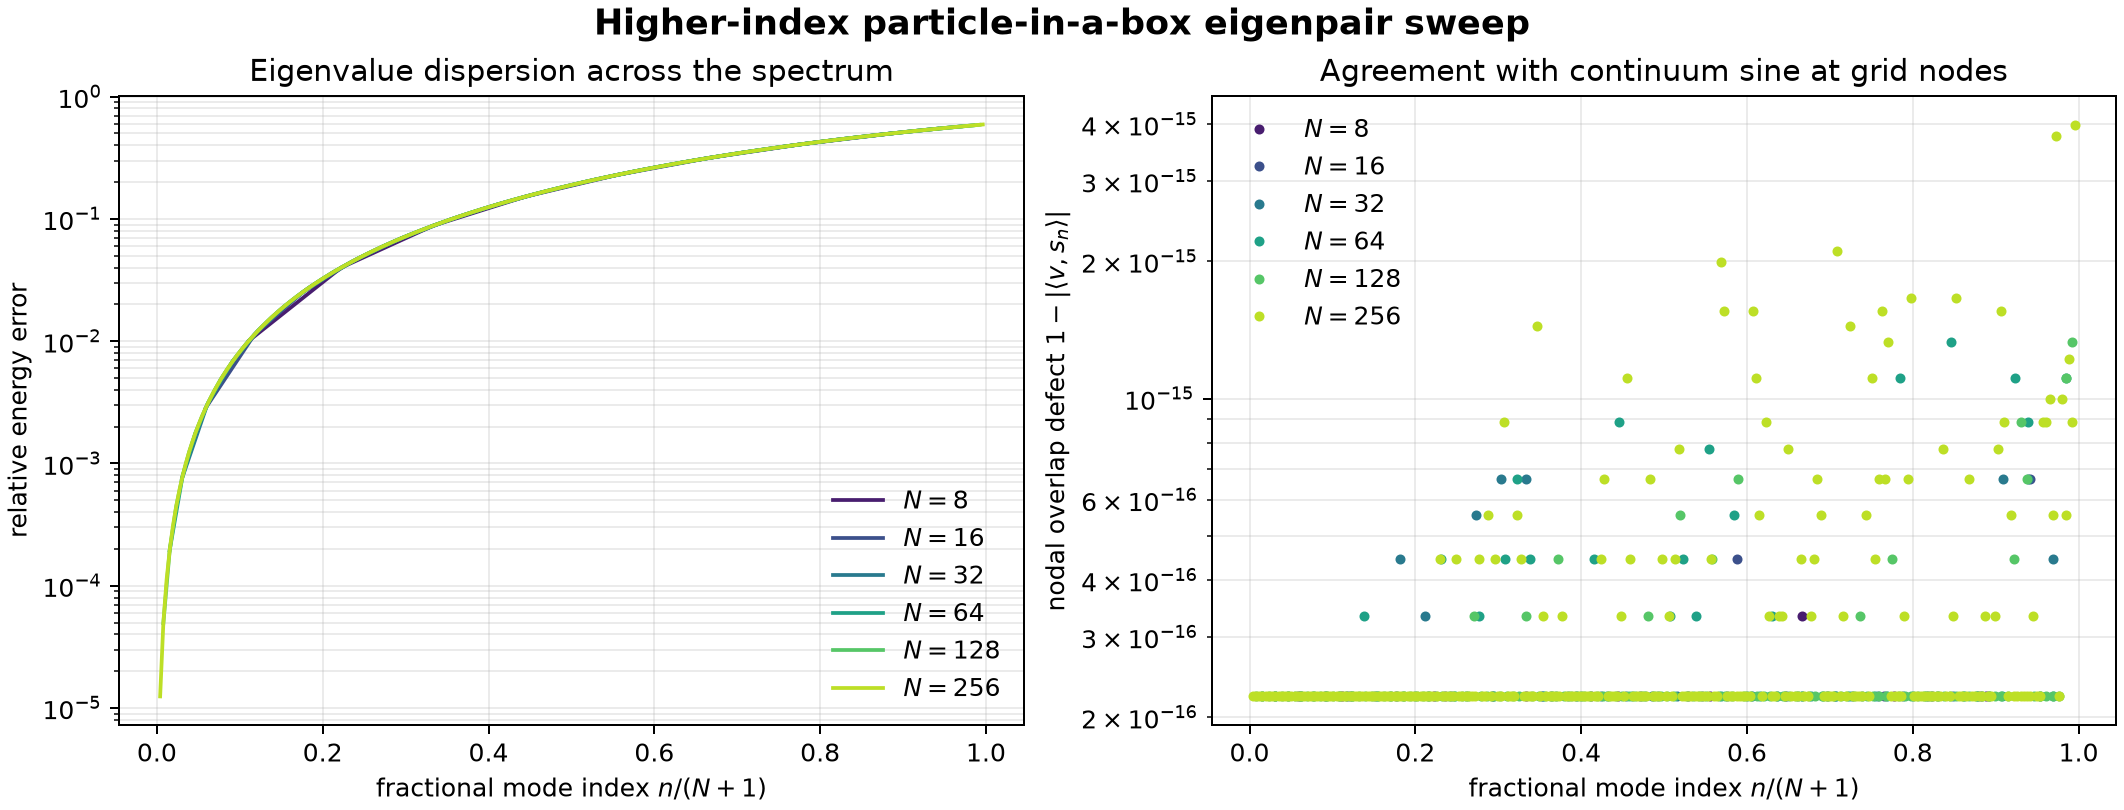
\includegraphics[width=\textwidth]{higher-eigenpair-sweep.png}
\caption{Full-spectrum eigenvalue dispersion and nodal overlap diagnostics.}
\label{fig:full-spectrum}
\end{figure}

\clearpage
\section{Dependence on matrix norm}

A residual does not have one universal magnitude. For a residual
$\mathbf R_h$, the same-grid ratios are
\begin{equation}
  \frac{\|\mathbf R_h\|_F}{\|\mathbf H_h\|_F},
  \qquad
  \frac{\|\mathbf R_h\|_2}{\|\mathbf H_h\|_2},
  \qquad
  \frac{\|\mathbf R_h\|_{\max}}{\|\mathbf H_h\|_{\max}}.
\end{equation}
Raw norms are retained but are not interpreted as convergence metrics across
changing spaces because matrix dimension and the $h^{-2}$ kinetic scale both
change.

The norm trends can be derived explicitly. Let
\begin{equation}
  c_h=\frac{\hbar^2}{2mh^2}.
\end{equation}
For the Dirichlet matrix,
\begin{equation}
  \|\mathbf H_h\|_F=c_h\sqrt{6N-2},
  \qquad
  \|\mathbf H_h\|_{\max}=2c_h,
\end{equation}
and
\begin{equation}
  \|\mathbf H_h\|_2
  =4c_h\cos^2\!\left(\frac{\pi}{2(N+1)}\right).
\end{equation}
The boundary residual consists only of the two corner entries of magnitude
$c_h$. Hence
\begin{equation}
  \|\mathbf B_h\|_F=\sqrt{2}\,c_h,
  \qquad
  \|\mathbf B_h\|_2=c_h,
  \qquad
  \|\mathbf B_h\|_{\max}=c_h.
\end{equation}
Its normalized ratios therefore satisfy
\begin{equation}
  \frac{\|\mathbf B_h\|_F}{\|\mathbf H_h\|_F}
  =\frac{1}{\sqrt{3N-1}}\longrightarrow0,
\end{equation}
\begin{equation}
  \frac{\|\mathbf B_h\|_2}{\|\mathbf H_h\|_2}
  =\frac{1}{4\cos^2[\pi/(2(N+1))]}\longrightarrow\frac14,
  \qquad
  \frac{\|\mathbf B_h\|_{\max}}{\|\mathbf H_h\|_{\max}}=\frac12.
\end{equation}
The apparently different graphical trends are thus exact consequences of the
different geometries encoded by the norms: aggregate Hilbert--Schmidt size,
worst-case Euclidean action, and largest coordinate entry.

\subsection{Unmatched compression}

\begin{table}[htbp]
\centering
\caption{Same-grid norm ratios for unmatched compression.}
\begin{tabular}{rrrr}
\toprule
$N$ & Frobenius & Spectral & Maximum entry\\
\midrule
8   & 0.9865 & 1.0000 & 0.9510\\
16  & 0.9994 & 1.0000 & 0.9940\\
32  & 1.0000 & 1.0000 & 0.9998\\
64  & 1.0000 & 1.0000 & 1.0000\\
128 & 1.0000 & 1.0000 & 1.0000\\
256 & 1.0000 & 1.0000 & 1.0000\\
\bottomrule
\end{tabular}
\end{table}

A fixed three-state retention discards nearly all of the increasingly resolved
operator norm. In the discrete eigenbasis, the unmatched residual has three
zero eigenvalues and the values $-E_{4,h},\ldots,-E_{N,h}$. It follows directly
that its spectral-norm ratio is one. Its squared Frobenius ratio is
\begin{equation}
  \frac{\|\widetilde{\mathbf R}_h\|_F^2}{\|\mathbf H_h\|_F^2}
  =1-
  \frac{\sum_{n=1}^{M}E_{n,h}^2}
       {\sum_{n=1}^{N}E_{n,h}^2},
\end{equation}
which approaches one for fixed $M$ as $N$ grows. The trend therefore records
what was excluded by the fixed-rank retention; it is not evidence for an
emergent potential and does not approach zero.

\subsection{Boundary realization}

\begin{table}[htbp]
\centering
\caption{Same-grid norm ratios for the boundary realization.}
\begin{tabular}{rrrr}
\toprule
$N$ & Frobenius & Spectral & Maximum entry\\
\midrule
8   & 0.2085 & 0.2578 & 0.5000\\
16  & 0.1459 & 0.2521 & 0.5000\\
32  & 0.1026 & 0.2506 & 0.5000\\
64  & 0.0724 & 0.2501 & 0.5000\\
128 & 0.0511 & 0.2500 & 0.5000\\
256 & 0.0361 & 0.2500 & 0.5000\\
\bottomrule
\end{tabular}
\end{table}

The Frobenius ratio decreases because two boundary couplings become small
relative to the aggregate norm of an $N\times N$ Hamiltonian. The spectral
ratio approaches 0.25, so worst-case Euclidean action remains a fixed fraction
of the Hamiltonian scale. The maximum-entry ratio remains 0.5 in the declared
grid basis. These statements are compatible because the norms answer different
questions.

\begin{figure}[p]
\centering
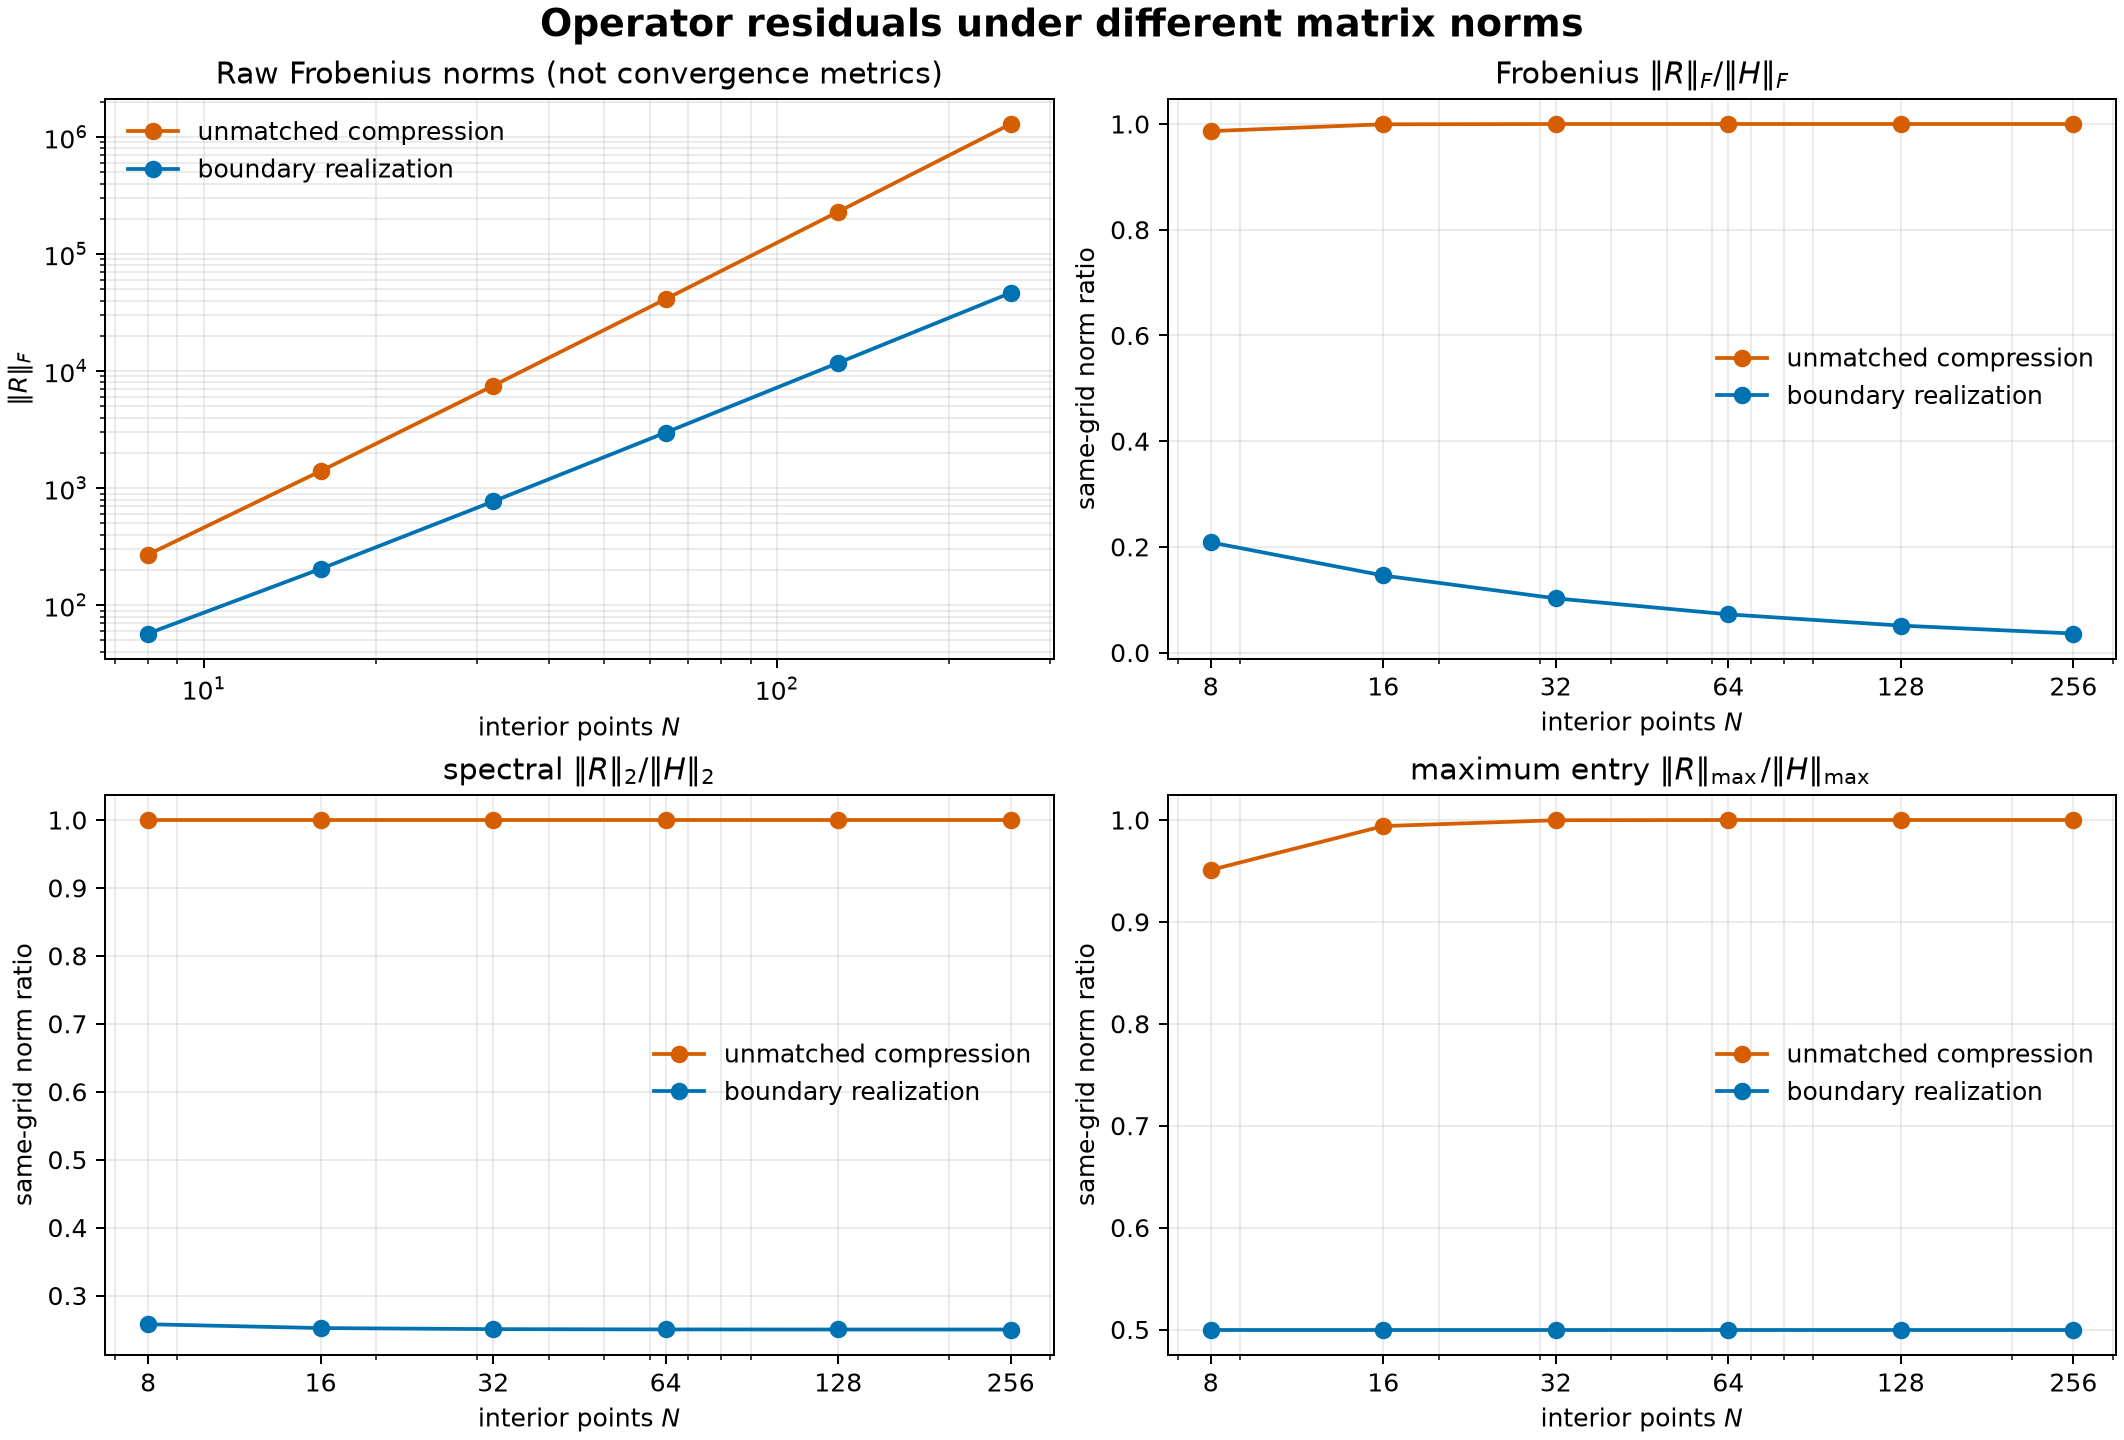
\includegraphics[width=0.94\textwidth]{operator-residual-norms.png}
\caption{Raw Frobenius norms and same-grid-normalized Frobenius, spectral, and
maximum-entry residual norms.}
\label{fig:operator-norms}
\end{figure}

The full-eigensystem algebraic residual matrix
\begin{equation}
  \mathbf H_h\mathbf V-\mathbf V\boldsymbol\Lambda
\end{equation}
has same-grid norm ratios below $10^{-15}$ throughout the series. This is an
eigensolver diagnostic only.

\begin{figure}[p]
\centering
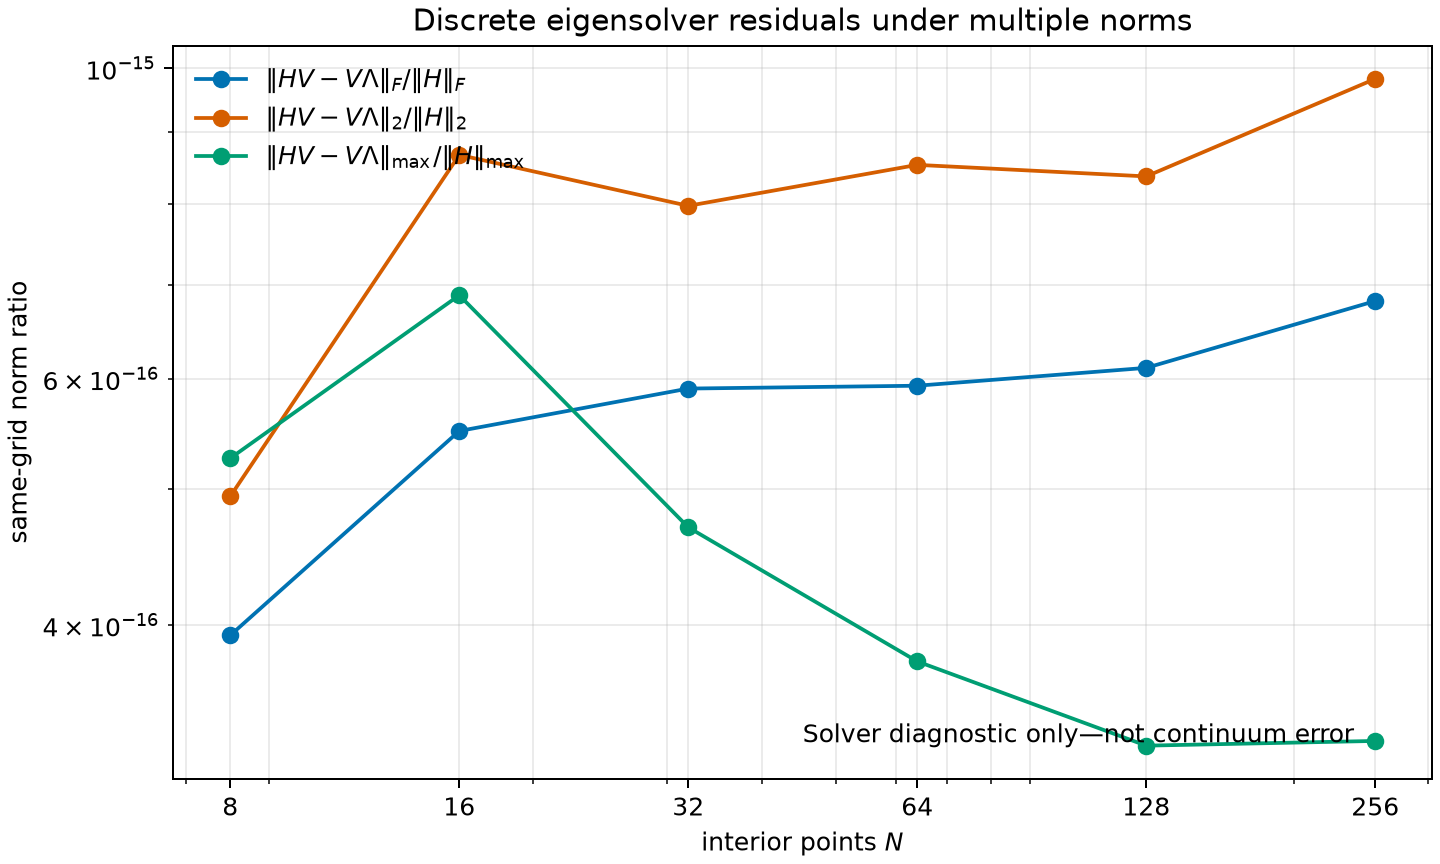
\includegraphics[width=0.88\textwidth]{eigensolver-residual-norms.png}
\caption{Algebraic eigensolver residual ratios under three matrix norms. These
are not continuum-error estimates.}
\label{fig:eigensolver-norms}
\end{figure}

\clearpage
\section{Residual identifiability}

The reduced Hamiltonian does not uniquely identify a kinetic--potential
partition. The ambiguity is structural rather than numerical. If one
admissible decomposition is
$\mathbf H_{\mathrm{red}}=\mathbf T_0+\mathbf R_{T_0}$, then every Hermitian
matrix $\mathbf K$ on the retained space generates another exact decomposition,
\begin{equation}
  \mathbf H_{\mathrm{red}}
  =(\mathbf T_0-\mathbf K)+(\mathbf R_{T_0}+\mathbf K).
\end{equation}
The set of decompositions is therefore an affine family unless prior physical
conditions restrict either term. On the $M=3$ retained coordinate space, the
declared physical box decomposition is
\begin{equation}
  \mathbf H_{\mathrm{red}}
  =\mathbf T_{\mathrm D,red}+\mathbf0.
\end{equation}
For a declared illustrative real-symmetric shift $\mathbf K$, the same matrix
also satisfies
\begin{equation}
  \mathbf H_{\mathrm{red}}
  =(\mathbf T_{\mathrm D,red}-\mathbf K)+\mathbf K.
\end{equation}
The physical decomposition reconstructs with zero Frobenius error. The shifted
decomposition reconstructs with error $1.11\times10^{-16}$. This agreement is
expected from the algebra and verifies only its finite implementation. The
second equality does not make $\mathbf K$ a physical potential. A physical
assignment would require independent justification of the shifted kinetic
reference and of the admissible structure of the remaining term.

\section{Dependence on the admissible model class}

The illustrative shift was fitted in Frobenius norm to four nested model
classes. If $\mathcal M_V$ is the chosen class, the unexplained residual is
\begin{equation}
  \mathbf E_{\mathcal M}
  =\mathbf K-\mathbf V_{\mathcal M}^{\star}.
\end{equation}
Under the Frobenius inner product, each fit is an orthogonal projection onto the
corresponding linear matrix subspace. The scalar fit retains only the mean
trace, the diagonal fit retains all diagonal entries in the declared basis, and
the tridiagonal fit additionally retains nearest-coordinate couplings. The
unrestricted real-symmetric class contains the target itself. This hierarchy
makes two points explicit: model-class restriction creates the informative
residual, and basis-dependent classes such as ``diagonal'' or ``tridiagonal''
are meaningful only after the retained basis has been identified.

\begin{table}[htbp]
\centering
\caption{Frobenius residuals after fitting the illustrative shift.}
\begin{tabular}{lr}
\toprule
Admissible model class & $\|\mathbf E_{\mathcal M}\|_F$\\
\midrule
Scalar identity & 1.9967\\
Diagonal in retained basis & 1.8561\\
Real symmetric tridiagonal & 0.5657\\
Arbitrary real symmetric & 0.0000\\
\bottomrule
\end{tabular}
\end{table}

The unrestricted class fits exactly by construction and is therefore
uninformative. Restricted classes leave different unexplained residuals. The
scientific inverse problem begins only after locality, range, symmetry,
differential form, parameter sharing, transferability, or another admissible
structure has been specified.

\begin{figure}[p]
\centering
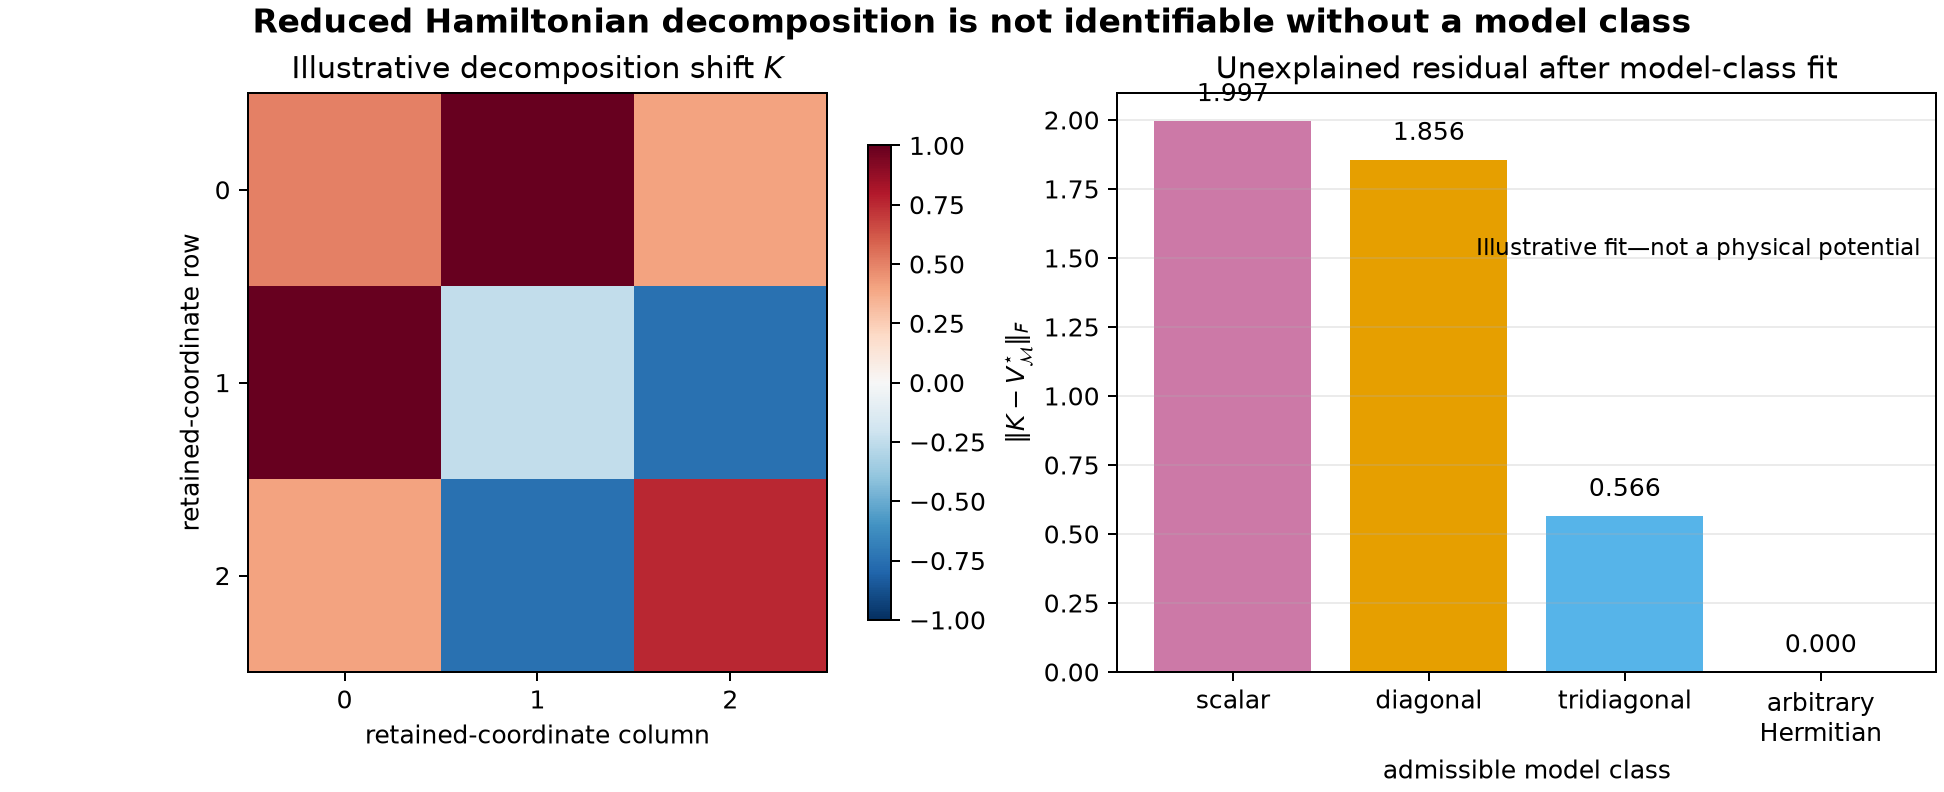
\includegraphics[width=\textwidth]{identifiability-model-classes.png}
\caption{Illustrative decomposition shift and model-class dependence of the
unexplained Frobenius residual. The shift is not assigned as a physical
potential.}
\label{fig:identifiability}
\end{figure}

\clearpage
\section{Discussion}

The calculations separate three error and interpretation questions that would
otherwise be easy to conflate. First, the algebraic residual
$\mathbf H_h\mathbf V-\mathbf V\boldsymbol\Lambda$ concerns solution of the
finite eigenproblem. Its near-roundoff magnitude shows that diagonalization is
accurate. Second, the difference $E_{n,h}-E_n$ concerns approximation of a
specified continuum eigenvalue by the finite operator. Its second-order decay
for fixed $n$ is a discretization statement. Third, an operator residual such
as $\mathbf H_{\mathrm{red}}-\mathbf T_0$ concerns a chosen decomposition. Its
physical meaning is not determined by either of the first two error measures.

The norm study sharpens this separation. The boundary residual is sparse and
therefore small relative to the aggregate Frobenius size of the growing
Hamiltonian, yet its spectral action remains one quarter of the Hamiltonian
scale asymptotically. Neither statement is more correct; each answers a
different question. A model-reduction criterion must therefore declare whether
it controls average matrix content, worst-case action, selected states, or
another operational quantity. Reporting an unlabeled norm would suppress this
choice.

The unmatched-compression calculation provides a complementary warning. Its
order-one normalized norm does not show that spectral retention has failed. It
shows that the retained and reference terms were subjected to different maps.
For observables restricted to the retained eigenspace, the discarded block may
be intentionally irrelevant; as a full-space operator subtraction, however, it
is necessarily large. The state space on which a claim is made is therefore
part of the claim itself.

Finally, the model-class experiment converts the nonuniqueness proof into a
finite calculation. Exact reconstruction by multiple decompositions is not a
competition between physical models: one alternative was introduced solely to
exhibit the affine ambiguity. Scientific content enters only when external
principles restrict the kinetic reference and potential class. In later
semiconductor reductions those restrictions may involve locality, symmetry,
range, shared parameters, or transferability, but this illustrative example
does not select among them.

\section{What the combined study establishes}

The calculated illustrative experiment establishes the following finite
statements under the retained inputs and binary64 implementation:
\begin{enumerate}
  \item The centered finite-difference spectrum agrees with its closed-form
        discrete oracle.
  \item Fixed-index eigenvalues converge at the expected second order once
        resolved.
  \item The growing full spectrum is not uniformly accurate.
  \item Consistent reduction gives the zero physical potential for the box.
  \item Unmatched reduction gives the negative discarded kinetic sector.
  \item The declared boundary subtraction gives a finite boundary-reference
        operator.
  \item Frobenius, spectral, and maximum-entry norms emphasize different
        aspects of the same residual.
  \item Accurate solution of the discrete eigenproblem does not imply
        continuum accuracy.
  \item The same reduced Hamiltonian permits distinct exact algebraic
        decompositions.
  \item The unexplained residual depends on the admissible model class.
\end{enumerate}

The central conclusion is not that one residual norm is preferable in every
circumstance. A residual can be interpreted only after the state spaces, maps,
reference operator, norm, and admissible model class have been declared.

\section{Limitations}

\begin{itemize}
  \item The cyclic closure is a declared finite comparison reference, not a
        unique continuum reference operator.
  \item Same-grid normalization does not align operators across changing
        numerical spaces.
  \item Fixed-mode convergence does not establish uniform spectral or operator
        convergence.
  \item Nodal eigenvector overlap does not establish continuum interpolation
        error.
  \item The illustrative shift $\mathbf K$ has no physical assignment.
  \item The model-class comparison uses a declared retained basis and
        Frobenius metric; changing either changes the fit.
  \item No result validates a material model or supplies evidence about
        silicon, DFT, Wannier localization, or impurity physics.
\end{itemize}

\section{Reproduction and retained evidence}

The exact commands are recorded in \texttt{README.md}. The retained evidence
consists of frozen JSON inputs, standalone calculation scripts, independent
verification scripts, retained JSON results, calculated graphics, software
identities, and SHA-256 checksums. Passing verification establishes agreement
with the stated finite mathematics and analytical oracles. It does not provide
scientific validation or human acceptance of a physical model.

\begin{thebibliography}{9}

\bibitem{bonneau2001}
G.~Bonneau, J.~Faraut, and G.~Valent,
``Self-adjoint extensions of operators and the teaching of quantum mechanics,''
\emph{American Journal of Physics}, vol.~69, no.~3, pp.~322--331, 2001.
\href{https://doi.org/10.1119/1.1328351}{doi:10.1119/1.1328351}.

\bibitem{angelone2024}
G.~Angelone, P.~Facchi, and M.~Ligab\`o,
``Classical echoes of quantum boundary conditions,''
\emph{Journal of Physics A: Mathematical and Theoretical}, vol.~57,
p.~425304, 2024.
\href{https://doi.org/10.1088/1751-8121/ad7428}{doi:10.1088/1751-8121/ad7428}.

\bibitem{strikwerda2004}
J.~C. Strikwerda,
\emph{Finite Difference Schemes and Partial Differential Equations}, 2nd~ed.
Philadelphia, PA: Society for Industrial and Applied Mathematics, 2004.
\href{https://doi.org/10.1137/1.9780898717938}{doi:10.1137/1.9780898717938}.

\end{thebibliography}

\end{document}
